%%%%%%%%%%%%%%%%%%%%% chapter.tex %%%%%%%%%%%%%%%%%%%%%%%%%%%%%%%%%
%
% sample chapter
%
% Use this file as a template for your own input.
%
%%%%%%%%%%%%%%%%%%%%%%%% Springer-Verlag %%%%%%%%%%%%%%%%%%%%%%%%%%
%\motto{Use the template \emph{chapter.tex} to style the various elements of your chapter content.}
\chapter{Chapter Heading}
\label{intro} % Always give a unique label
% use \chaptermark{}
% to alter or adjust the chapter heading in the running head

\begin{abstract}
Security architectures can pose complexity and cast doubt. How can we be certain that the solutions we have acquired are adequate? How can we know they are configured properly to cover the many vectors of a cyberattack? Much of the industry at large has adopted the use of MITREs \textbf{Adversarial Tactics, Techniques, and Common Knowledge Database (ATT\&CK)} Framework to help objectively assess those solutions and their coverage of an attacker's than an environment is most likely to encounter. This chapter aims showcase to defenders the benefits of learning from the mistakes of others, how to use the MITRE ATT\&CK framework to evaluate their blind spots, and understand through demonstrations how to better defend infrastructure through the use of coverage mapping, orbital scanning, and Caldera.
\end{abstract}

\section{The Importance of Cyber Threat Intelligence and the MITRE ATT\&CK Framework}

\begin{quote}
    "I must not fear. Fear is the mind-killer. Fear is the little-death that brings total obliteration. I will face my fear. I will permit it to pass over me and through me."
    -Frank Herbert, Dune
\end{quote}
Before an organization can effectively defend its environment, it must first understand the methods, tools, and tactics that real-world adversaries employ. One of the most valuable resources available for this exact purpose is the MITRE ATT\&CK Framework, a globally recognized knowledge base that systematically documents how cyber adversaries operate.

The MITRE Corporation
The MITRE Corporation is a not-for-profit organization that operates multiple \textit{Federally Funded Research and Development Centers (FFRDCs)} in the United States. Established to bridge the gap between government, industry, and academia, MITRE engages in a wide range of public-private partnerships, with a strong focus on cybersecurity innovation. It works closely with U.S. government agencies, critical infrastructure sectors, and private industry to research, design, and improve systems that safeguard national and organizational security.

Cybersecurity professionals may already be familiar with MITRE as the organization responsible for maintaining the \textit{Common Vulnerabilities and Exposures (CVE)} database-a publicly available list of known security vulnerabilities used worldwide for vulnerability management, patch prioritization, and security research.

Defining the MITRE ATT\&CK Framework
Pronounced as \textit{"MITE-ER ATTACK,"} the MITRE ATT\&CK stands for \textit{Adversarial Tactics, Techniques, and Common Knowledge.} It originated in 2013 as an internal MITRE project to document the \textit{Tactics, Techniques, and Procedures (TTPs)} that Advanced Persistent Threats (APTs) were using to compromise and persist within WIndows enterprise networks. Over time, ATT\&CK evolved into a globally accessible knowledgebase covering not just the Windows operating system, but also macOS, Linux, mobile platforms, cloud environments, and \textit{Industrial Control Systems (ICS).}

The framework organizes adversary behaviors into a series of \textit{tactics} (the adversary's technical goals during an intrusion) and \textit{techniques} (the specific methods used to achieve those goals). Each technique entry in ATT\&CK is enriched with fine details such as:
Technical descriptions and examples of real-world usage.
Mappings of real-world APTs and nation-states back to TTPs frequently used.
Detection guidance and telemetry sources.
Mitigation recommendations.
References to documented threat actor activity.

Why the MITRE ATT\&CK Framework Matters
The ATT\&CK framework matters significantly because for one, it provides you a structured, knowledge-based approach to understanding and mitigating cyber threats correctly and effectively. No guessing games. And secondly is because it has helped many organizations improve their security stances by offering a common language for describing attacker behavior. This effectively, in turn, enables better communications channels between security teams, which in turn guarantees a more effective response to when a breach or threat presents itself because we are all "speaking the same language." Confusion, for the most part, is eliminated.




\section{Exploitation: Pulling the Proverbial Trigger
}If delivery is the act of smuggling the weapon into the room unnoticed, exploitation is about pulling the proverbial trigger. At this stage is when the attacker executes the payload using the vulnerability identified back in the reconnaissance phase and actively abuses to gain a toehold. And for us, it means every prior prevention layer has failed to keep the weapon out.
The type of exploit used depends entirely on the chosen delivery vector and the specific weakness it is designed to target. For example:

\begin{itemize}
    \item An email-borne weapon might execute a malicious macro in a document.
    \item A poisoned website might trigger a browser or plugin exploit.
    \item A USB-delivered payload could auto-run malware or drop an infected rootkit.
\end{itemize}

From the attacker's view, the objective here is to ultimately gain control—whether that means executing arbitrary code to escalate privileges, or installing a persistent backdoor. In many cases, exploitation also involves disabling security tools or altering configurations to make the attacker's life easier later.
For defenders, this is a critical choke point. The best protection is to remove the attacker's opportunity before they get this far. Some recommendations to achieve this may include, but are not limited to:

\begin{itemize}
    \item Keeping all operating systems (OS), applications, and plugins patched.
    \item Disabling unnecessary features (like macros) wherever possible.
    \item Running updated endpoint protection capable of detecting both known and behavior-based threats.
\end{itemize}

Using Endpoint Detection and Response (EDR) to spot unusual execution patterns in near-real-time. Once the exploit is launched, the attacker's goal is crystal clear: establish control, expand access and reach, and position themselves for the next stage of their operation. That may involve compromising additional systems, capturing higher-privilege credentials, or gaining administrative rights to dominate the environment.

If the exploit leverages a known vulnerability, there is still a slim chance to blunt its impact with remaining safeguards such as Data Execution Prevention (DEP)—a security feature in Windows, Linux, and macOS that blocks code executions from non-executable memory regions-and anti-exploit protections embedded in modern antivirus solutions.

Other defensive measures at this point are containment-oriented. Automatic privilege escalation and de-escalation policies can greatly limit how long an attacker can retain elevated rights. Sandboxing can isolate suspicious processes or files in a controlled environment, allowing analysts to safely observe the exploit's behaviors, extract Indicators of Compromise (IOCs), and prepare defenses against similar attacks in the future.

It is important to remember: exploitation is rarely the endgame. The real objective is to deepen access, to move closer to core systems, data, and privileges that matter most. If exploitation succeeds, the attacker has then transitioned from "outside" to "inside." At this point, they are no longer just probing-they have an operational presence in the environment. From here on, the campaign moves into the next phase: \textbf{Installation}.

\section{Installation: Making It Stick}
For the attacker, exploitation is just the opening act. The real payoff comes when they can stay remaining quiet, invisible, and for as long as it takes to achieve their mission, or until they are rudely booted from the network.

Persistence can take many forms such as hidden services, malicious scheduled tasks, registry modifications, startup scripts, or implanted backdoors. A skilled adversary does not always rush, and as we all know too well that rushing anything delivers mistakes. An adversary might restart the entire kill chain internally, running fresh reconnaissance now that they have landed inside, probing for additional targets and higher-value systems they can breach, or use as pivoting points to access other parts of the restricted network.

The dual objectives in this phase are clear:
\begin{enumerate}
    \item Maintain uninterrupted access despite restarts, patches, or credential resets.
    \item Escalate privileges to gain broader and deeper control over the environment.
\end{enumerate}

This is also the point where traditional, signature-based detection struggles. Advanced Persistent Threats (APTs) often use subtle, custom-built techniques that will not trigger classic intrusion detection rules. Zero day exploits and fileless malware can hide in plain sight.

It is at this point that Endpoint Detection and Response (EDR) become vital. Unlike basic Endpoint Protection Platforms (EPP) that focus primarily on prevention, EDR is designed to detect and respond when prevention has failed. A capable EDR solution can:
\begin{itemize}
    \item Identify malicious activities that have bypassed initial security layers.
    \item Contain the infection before it spreads.
    \item Provide forensic data in near-real-time for investigation and remediation.
\end{itemize}

Once an infected system is confirmed, restoration to a known stable state becomes the defender's priority. That means verified clean backups, secure reimaging, and validation that the attacker's persistence mechanisms have been completely eradicated. Skipping this step risks leaving hidden toeholds that can reignite the compromise at a later point in time.

From here, an attacker with persistence and elevated privileges is positioned to take the next steps: internal reconnaissance, lateral movement, and ultimately, the completion of their mission.

\section{Command and Control: The Attacker's Lifeline}
By the time the operation reaches this phase, the attacker has accomplished something significant: the target system is compromised, persistence has been established, and the door is propped wide open. If the earlier steps have been executed cleanly, their toehold will survive any removal efforts from defenders such as patching, rebooting, and remedial efforts deem unsuccessful.

From here, the compromised information system can serve two primary roles. It might be used immediately to carry out the attacker's mission: exfiltrating data, sabotaging services, or manipulating systems. Or it may simply sit, quietly awaiting further instructions from a Command and Control (C2) server, acting as a sleeper agent until the moment to strike is right.

C2 channels are the attacker's covert lifeline. They all remote operators to conduct activities such as:
\begin{itemize}
    \item Push and introduce new payloads or tools into the compromised environment.
    \item Issue commands for reconnaissance, lateral movement, or privilege escalation.
    \item Exfiltrate stolen data in controlled bursts to avoid detection.
\end{itemize}

The best defensive posture at this stage is to focus on detecting anomalies and limiting the attacker's reach and maneuvering space.
\begin{itemize}
    \item Network segmentation ensures that even if one system is compromised, the attacker cannot freely roam the entire environment.
    \item Application segmentation enforces restrictions at the service and workload levels, narrowing what can be reached from the infected host(s).
\end{itemize}

Detection tools should be fine-tuned to look for changes in normal network traffic patterns and behaviors (drawn from previous "normal" baselines of network traffic activities).
\begin{itemize}
    \item Sudden spikes in data or ingress and egress network traffic being sent to or from external IP addresses.
    \item Transfers to geographic regions outside normal business activities.
    \item CPU or memory spikes at odd hours that do not match expected usage times.
\end{itemize}

Lateral movement goes hand-in-hand with privilege escalation and is considered the art of pivoting from one compromised system to another. Lateral movement is also often the attacker's next move from here. It is how they deepen their reach, their access, compromise higher-valued assets, and position themselves to strike and hit their true target. Once inside, they may use tools like Mimikatz to harvest credentials, or exploit trusts between information systems to leapfrog across the networks.

Proactive defenses really shine here. Breach and Attack Simulation (BAS) platforms can emulate realistic C2 activities, lateral movements, and data exfiltration scenarios inside your environment. By running these controlled tests, defenders can better identify their blind spots, validate detection capabilities, and fine-tune their response procedures before facing an actual adversary.

At this point, the attacker's tether to the victim is strong. Breaking it, severing that C2 covert communications channel, is essential to disrupting their campaign. If left unchecked, the next and final stage is where the operation's ultimate objective is realized.

\section{Actions on Objectives: Completing the Mission}
At this stage, the attacker's work has come full circle. The information system is fully infected and compromised, persistence has been established and is in secured place, and Command and Control covert channels are live. Now comes the end-game, where the attacker's actions are taken to fulfill the mission.

The exact nature of these actions is driven entirely by the attacker or what the organizational objectives and goals are for the mission. For some attackers, motivation is driven by financial gain-siphoning payment data, holding systems for ransom, or selling access to dark web marketplaces and forums. For other attackers, it is driven by political or strategic espionage, quietly collecting intelligence over weeks, months, and sometimes even years! And sometimes, the goal is simply just to pivot around, to move laterally across the network until a higher-value target has been discovered and identified.

Lateral movement is common here. The attacker may initiate a new internal reconnaissance phase, mapping systems, enumerating accounts, and probing for weaknesses in the network core. Each successful hop can lead them closer to sensitive assets, databases, domain controllers, or proprietary intellectual property or trade secrets.

The COVID-19 pandemic accelerated this risk ten-fold. Practically overnight, the network perimeter expanded far beyond the office walls, stretching into home offices, personal devices, and often poorly secured internet, WiFi, and Bluetooth connections. Remote work was not just for employees; system and network administrators, the very people tasked with defending the crown jewels, were suddenly performing their duties from spare bedrooms and kitchen tables.

Under normal circumstances-although, in cybersecurity, "normal" is a relative term-part of an administrator's morning routine or checkbox from a 'daily tasks list' might involve a quick visual inspection of the servers-checking status lights, scanning for unusual messages that marquee on server LED screens, or simply walking the data center floor to spot anything suspicious. These small, routine habits form an informal but effective layer of security.

When those "eyes on" spot checks vanished, attackers noticed. They understood-or outright knew-that the defenders were now remote (for the most part), and that physical systems no longer had a Big Brother. This absence quickly became a golden opportunity for attackers as this newfound absence introduced a larger and widened attack surface, turning the physical infrastructure into a more tempting attack playground. Without boots on the ground, malicious activities at the hardware level or in the data center's immediate environment could go unnoticed for far longer than before.

\section{Zero Trust}
Zero trust security is a cybersecurity framework that enforces strict identity verification for every user and device attempting to access resources on a network. Zero trust assumes that no user or device is inherently trustworthy, regardless of whether they are inside or outside of the network perimeter. It is a security model that requires continuous verification and authentication for every access request, implementing a \textit{"never trust, always verify"} approach to enhance security. This model moves away from the traditional perimeter-based security, where trust was assumed within the network, and instead focuses on granular access control and continuous validation of identities and devices.

Furthermore, the core philosophy assumes that potential threats exist both internally and externally, meaning neither users nor systems should be given implicit trust. A key principle of this approach is \textbf{least-privilege access}, granting individuals only the minimum permissions necessary to perform their duties (e.g., fulfill obligations and expectations specific to their role). This, in turn, reduces unnecessary exposure to sensitive information systems and helps to thwart privilege escalation attempts, a critical stage in many attack chains.

Zero trust operates using several key principles:
\begin{itemize}
    \item Verify every request: All users and devices must authenticate and be authorized before accessing any resources.
    \item Least privilege: Users receive only the minimum access necessary to perform their duties, reducing the blast radius of any compromise.
    \item Micro-segmentation: Security perimeters and boundaries are broken into smaller, isolated zones, limiting lateral movements and enforcing \textit{"privacy by default"} with applications.
    \item Multi-Factor Authentication (MFA): More than one form of verification is required; passwords alone are insufficient.

\end{itemize}

Zero trust architectures also incorporate \textit{micro-segmentation,} the practice of dividing the network into smaller, isolated zones so that access to one segment does not inherently grant access to other surrounding networks. When implemented and enforced at the application level, properly configured micro-segmentation inherently supports the \textit{privacy by default} principle by ensuring that access and data exposure are limited to only what is strictly necessary.

\textit{Multi-Factor Authentication (MFA)} is another core security control, requiring users to provide more than one form of verification before access is granted. Often referred to as triple authentication, MFA is based on the principle of validating of identity verification and validation. The model comes from the established three authentication factor categories:

1. \textit{Something you know:} Knowledge-based credentials such as passwords, PINs, or answers to security question challenges.
2. \textit{Something you have:} Physical or virtual items such as security tokens, smart cards, or mobile authentication apps.
3. \textit{Something you are:} Inherent biometric traits like fingerprints, facial recognition, or iris scans (hello Cyberdyne Networks).

Adopting zero trust doesn't completely eliminate risk as nothing ever will, but it dramatically reduces an attacker's ability to escalate privileges and reach their ultimate objectives whatever they may be.

TL;DR: in a zero trust model, no entity is automatically trusted; every request for access must be authenticated and authorized. No questions asked. No if's, and's, or but's.

\section{The MITRE ATT\&CK Framework}
For defenders, the \textbf{MITRE ATT\&CK} knowledge base is an invaluable tool. It catalogs known adversary tactics and techniques, mapping them to real-world threat behaviors. It also provides guidance on detection, mitigation, and response strategies tailored to specific attack patterns. Organizations can use it as the foundation for threat modeling, incident response planning, and security control validation.

When attackers reach this phase, the clock is ticking. Every second matters. Rapid detection, containment, and remediation can still prevent catastrophic damage — but only if the defenders have prepared for this moment long before it arrives.




For defenders, the MITRE ATT\&CK knowledge base is a valuable resource, cataloging adversarial \textit{Tactics, Techniques, and Procedures (TTPs)} and offers guidance on detection and mitigation strategies.
\begin{figure}
    \centering
    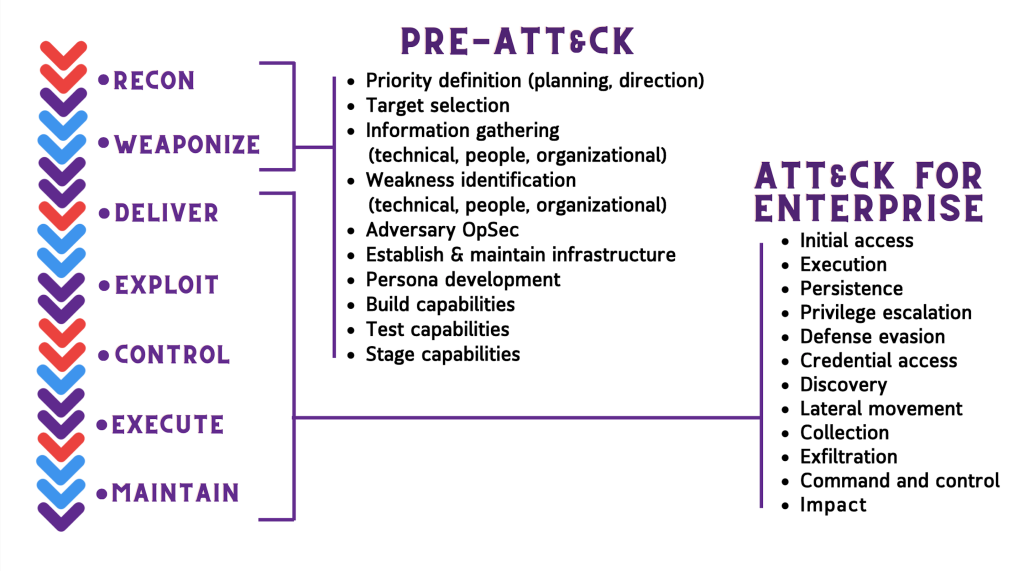
\includegraphics[width=0.75\linewidth]{att&ck.png}
    \caption{MITRE ATT\&CK Framework}
    \label{fig:placeholder}
\end{figure}

\section{Beyond Prevention: Building a Full-Spectrum Security Program}
As we have seen so far, prevention alone is not enough to stop a determined adversary. Defenders and organizations need a balanced security program that combines prevention, detection, and response into a continuous cycle. A well-structured offensive security program is one of the most effective ways to strengthen security posture and identify weaknesses across all three areas.

This approach ensures not only that security controls are effective, but also that the security staff have the skills and readiness to respond appropriately when incidents occur. It goes well beyond penetration testing. While pentesting is valuable, it is limited in scope and-when treated as the sole focus-can foster a false sense of security. Compliance checks alone are not equally sufficient enough either.

That said, launching an offensive security program comes with challenges, as most endeavors do, with the most immediate being executive buy-in. One way to build support is to start small: conduct a targeted penetration test on carefully chosen applications or network segments, prioritized through a risk assessment. The results can highlight quick wins, particularly high-risk issues, and help justify further investment.

For many organizations, the program may begin as a "one-man" operation supported by specialized external providers and experts. Over time, as the value and business impact become clear, the team can grow organically. Without demonstrating that value to leadership, the initiative risks remaining an underfunded side project rather than a true success story.

\section{Red Teaming: The Sharpest Pre-Compromise Tool}

When it comes to proactive, pre-compromise testing, Red Teaming stands out. It is a goal-based adversarial exercise in which a skilled team simulates a real-world attack against predefined objectives. Red teams use the same tools, techniques, and methods that genuine adversaries employ-often in long-form engagements that involve reconnaissance, exploitation, lateral movement, and persistence.

Unlike traditional penetration tests, Red Teaming is interactive and iterative, mirroring the ebb and flow of a live intrusion. Its purpose is to access whether the organization can prevent such attacks from succeeding, detect them if they do, and respond effectively to restore normal operations. Pairing a red team with a blue team (the defenders) provides the most thorough end-to-end review of the organization's true security readiness.

Because modern threats are increasingly becoming more and more complex as the days pass, defenders need a solid way to anticipate attacker behavior. Few organizations have the resources to defend against every possible threat vector. Zero day vulnerabilities, in particular, can bypass signature-based detections entirely. Attempting to address these without a structured methodology is a recipe for failure.

Incident responder and triage analysts must have a tried and true repeatable methodology for identifying and mitigating unknown threats to safeguard their most critical assets. Understanding the threat landscape is only half of the battle. The better we understand how our organization can be attacked, the better we can design and deploy effective countermeasures. After all, you can't protect what you don't know is out there.

\section{Threat Modeling and Attack Trees}
Threat modeling is the process of visualizing and analyzing all the ways in which an adversary might target an environment. Now, this is thinking like your adversary, or adopting an adversarial mindset to the max. One of the most effective tools for this is the attack tree. This structured model puts the defender in the attacker's shoes, mapping out the possible pathways to a given goal.

The root of the tree represents the attacker's ultimate objective, for example, "Access customer data" or "Disrupt business goals." Branches represent sub-goals or intermediate states, while leaf nodes represent concrete attacker actions. Nodes can be defined as:
Root node: The attacker's primary goal
OR node: Only one child action is required to succeed
AND node: All child actions must succeed
Leaf node: The final, concrete action taken by the attacker

To build an attack tree, ask yourself questions, such as these:
What would be the attacker's goal in our environment?
What would be the impact or range of destruction the attack can inflict the further into the network it go?
What attacks could be used against these areas?
What steps are required to start and finish each attack, and what is the attack's ultimate goal or objective?
Do there exist alternatives to achieve the same step twice?

Attack trees are not limited to digital threats-they can also model physical and hybrid attacks. For instance, an attacker might bypass digital controls by exploiting physical vulnerabilities: leaving an infected USB stick in a parking lot, tailgating into a secured facility, or tampering with on-site hardware, such as server or network appliance cables, or power outlets to cause disruptions.

Let us consider a simple example. Let us say that we want to analyze unauthorized physical access to one of our secured buildings. The root node would be "Gain Unauthorized Physical Access." From there, we would map possible entry points and the steps required for each, refining until each branch ends in trivial, actionable steps.

By visualizing the attack surface in the same manner as your adversarial opponent, you can identify weak points-both technical and non-technical-and design targeted countermeasures that will produce results-winning ones at that.

\subsection{Attack Tree Example-Goal: Gaining Unauthorized Physical Access}

\textbf{Root Node:} Gain Unauthorized Physical Access to Secured Building

\textbf{Branch 1-Tailgating (OR)}
\begin{itemize}
    \item Follow (or piggyback) an employee into the building without using credentials \textbf{(OR)}
    \begin{itemize}
        \item Blend in with a group entering
        \item Carry packages to appear as a delivery person
        \item Pretend to have a conversation with an employee
        \item Take advantage of busy entry times (shift changes, lunch rush)
    \end{itemize}
\end{itemize}

\textbf{Branch 2-Social Engineering (OR)}
\begin{itemize}
    \item Convince security or reception to grant entry \textbf{(OR)}
    \begin{itemize}
        \item Impersonate an employee who "forgot their badge"
        \item Claim to be a contractor or vendor
        \item Present a forged work order or service ticket
    \end{itemize}
\end{itemize}

\textbf{Branch 3-Exploiting Physical Weaknesses }(OR)
\begin{itemize}
    \item Bypass or tamper with entry controls \textbf{(OR)}
    \begin{itemize}
        \item Pick a door lock
        \item Use a stolen or cloned access card
        \item Exploit door mechanical failures (e.g., misaligned latch)
        \item Force the door open after authorized user exits (door not fully closed)
    \end{itemize}
\end{itemize}

\textbf{Branch 4-Using Unsecured Entry Points (OR)}
\begin{itemize}
    \item Access via less monitored points \textbf{(OR)}
    \begin{itemize}
        \item Loading dock or delivery entrance
        \item Emergency exit doors propped open
        \item Rooftop or maintenance access points
        \item Windows left unlocked or open
    \end{itemize}
\end{itemize}

\textbf{Branch 5-Inside Assistance (OR)}
\begin{itemize}
    \item Gain help from an insider \textbf{(OR)}
    \begin{itemize}
        \item Disgruntled employee grants entry
        \item A bribed or coerced staff member provides access credentials
        \item Insider temporarily disables entry alarms
    \end{itemize}
\end{itemize}

\begin{figure}
    \centering
    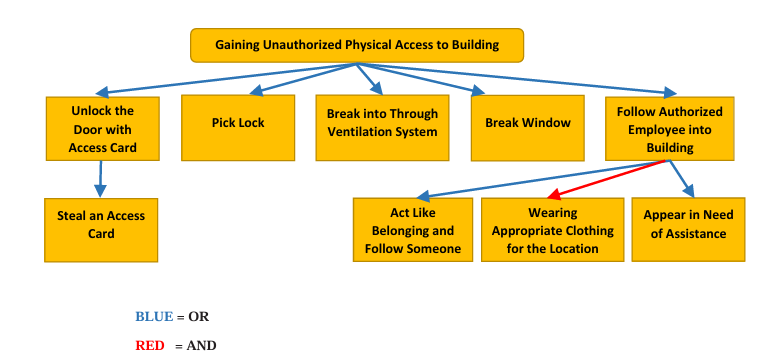
\includegraphics[width=0.75\linewidth]{attacktree.png}
    \caption{Figure 2. Attack Tree Example-Gain Unauthorized Physical Access to Secured Building}
    \label{fig:placeholder}
\end{figure}

\section{Linking the Cyber Kill Chain to Attack Trees}
If we place the attacker's \textbf{ultimate goal} at the top of the Cyber Kill Chain and connect each of the chain's seven phases beneath it, what we get begins to look very much like an attack tree. Each phase of reconnaissance, weaponization, delivery, exploitation, installation, Command and Control, and actions on objectives becomes a branch leading toward the goal.

Taking this step further, incorporating the MITRE PRE-ATT\&CK and MITRE ATT\&CK frameworks can enrich these trees by mapping real-world adversarial Tactics, Techniques, and Procedures (TTPs) to each branch. This allows defenders to visualize an attacker's modus operandi in detail, identifying points where detection or disruption is possible.  The MITRE knowledge bases are invaluable for this exact purpose, and there is no reasonable excuse for not leveraging them when building attack trees. Importantly, these trees must account for both physical and digital logical threats, as hybrid attack pathways are common in real-world attack campaigns.

\section{The OODA Loop: A Decision-Making Framework for Threat Analysis}
One challenge in constructing attack trees is determining which threats to prioritize and how to define the goals. In situations where uncertainty is high, the OODA Loop-Observe, Orient, Decide, Act-can be an effective tool for making decisions quickly and staying ahead of an adversary. Originally developed for military strategies, the OODA loop is a learning and decision-making cycle that enables faster adaptation than one's opponent.

\subsection{Observe}
Effective observation begins with \textit{situational awareness}. This means understanding your operational environment in its entirety-the current state of your systems, the capabilities and likely intentions of your adversaries, and the broader physical, technical, and even organizational context. In threat intelligence or threat hunting, observation is essentially the \textit{data collection phase}, where all available information is gathered without drawing any conclusions.

\subsection{Orient}
Orientation is the most critical phase of the loop. Here, the objective is to identify mismatches or errors in previous assumptions, blind spots in detection, or flaws in the adversary's understanding of your environment. In threat hunting, this means analyzing the collected data to define a set of relevant threats, determining how they might manifest under certain circumstances or different scenarios, and exploring possible mitigation. If uncertainty remains high, devote more time and resources to orientation. The goal is to develop and validate models or concepts \textbf{before} they are needed in live operations, and ensure confidence in their effectiveness.

\subsection{Decide}
In this phase, decision-makers form a hypothesis: a prediction of the most effective course of action based on the current model and understanding. This decision represents the best-informed guess on how to respond to a given threat scenario.

\subsection{Act}
The action phase tests the hypothesis in the real environment. If the model holds, the response is effective; if not, the loop starts again with new observations feeding into the next cycle. Ideally, multiple courses of action or controlled experiments are run in parallel to identify the optimal approach more quickly.

The OODA loop is powerful because of its speed and adaptability. In competitive or hostile environments, the side that can run consecutive OODA cycles faster-adapting more quickly than its opponent-will prevail. The "Orient" phase shapes not just how and what we observe, but also how we decide and act, making it the central lever of the loop.

\section{Red Teaming}
As a red teamer, you are playing the role of the "devil's advocate."

Red teams are indispensable for testing emerging operational concepts and challenging existing security measures. A Red Team's sole purpose is simple yet critical: \textbf{to identify weaknesses before the real adversaries exploit them.}

\subsection{Purpose and Value}
Red teaming provides defenders, blue teamers, security teams, and organizations with a realistic, adversary-focused assessment of their standing defensive capabilities. It is the \textbf{only means to accurately evaluate how security controls and measures withstand real-world attack scenarios.} By simulating sophisticated threat actors, Red Teams offer direct insight into whether investments in cybersecurity are paying off in measurable resilience.

Key outcomes of effective Red Teaming include:
Smarter decision-making under realistic threat conditions.
Risk reduction by identifying vulnerabilities that traditional testing misses.
Preparation for the unexpected, including previously unconsidered attack pathways.

In essence, Red Teams help answer the fundamental question:
\textit{"If we were attacked tomorrow, how would we fare?"}

\subsection{Role and Approach}
A mature Red Team does more than just execute attacks-it \textbf{challenges core assumptions} and evaluates the organization's security posture from an attacker, or attacking perspective. This often includes examining attack plans, strategies, and security controls under different hypotheses, producing alternative threat scenarios, and exposing gaps in both technical and procedural defenses.

Effective Red Team operations rely on \textbf{critical and creative thinking}. Members must not only understand the systems and processes in scope but also be able to approach problems from unconventional angles-mirroring the adaptability of real attackers.

\subsection{Essential Attributes for Red Team Members}
+When forming or expanding a Red Team, the following competencies and traits should be prioritized:
Adversarial mindset: Ability to see systems and defenses through the lens of an attacker.
Imagination-Freedom of thought to design unconventional attacks.
Self-awareness: Understanding both the enemy and one's operational limitations (\textit{adopted from Sun Tzu).}
Operational environmental knowledge: Familiarity with critical systems, variables, and decision-making processes.
Experience in cyber wargaming: To include experimentation and simulation best practices.
Confidence to challenge the status quo: Willingness to question assumptions.
Effective communication: Ability to report findings and recommendations.
Leadership and facilitation skills: Guiding engagements and ensuring cohesive team functions.

\section{Operating Principles}
For a Red Team to be truly effective, several structured and procedural requirements must first be met:
Operate with a predefined objective aligned to organizational risk policies.
Maintain independence from the Blue Team while ensuring adequate interaction for mutual learning experiences.
Possess full support from executive leadership to ensure access, scope coverage, and authority.
Adhere strictly to surrounding laws, regulations, organizational policies, and operating procedures, and defined Rules of Engagement (ROE).
Help identify adversary deception and denial strategies.
Assist defenders in assessing confidence levels in their detection and response data.

Trust is paramount. Red Teams handle sensitive data, and in the wrong hands, this intelligence could be catastrophic for the organization.

\section{Key Responsibilities of Red Team Operators}
A well-functioning Red Team will:
1. Test defensive effectiveness against advanced, persistent, and opportunistic threats.
2. Improve incident response capabilities by simulating real-world attack chains.
3. Evaluate internal standards and practices, identifying areas for Blue Team performance optimization.
Identify and mitigate high-impact vulnerabilities before adversaries do.
Execute realistic attack scenarios to obtain access, extract sensitive data, and assess potential business impacts.
Produce actionable reports that detail vulnerabilities, exploitation steps, and recommended avenues for mitigation.
Enhance organizational strategies, creating a roadmap for long-term security improvements and enhancements.
Educate defenders and leadership on newly  evolving or emerging threats and best practices.

\begin{figure}
    \centering
    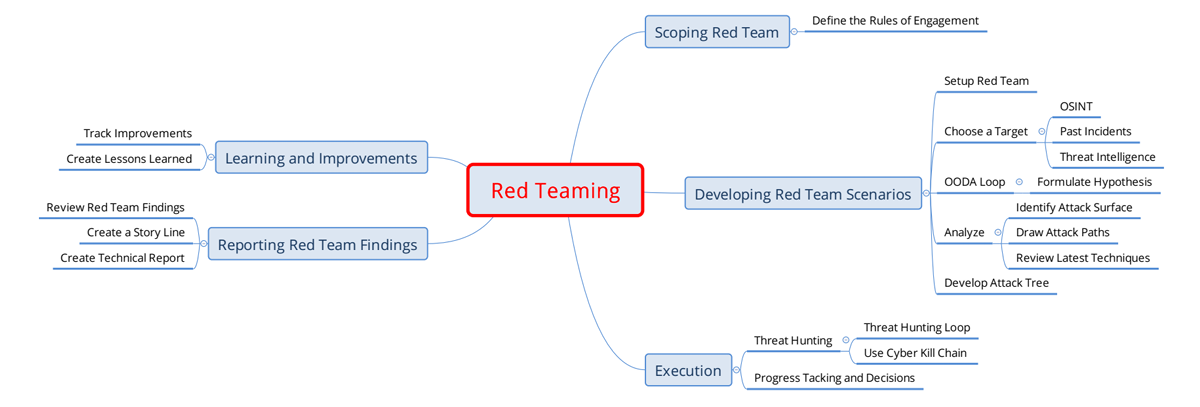
\includegraphics[width=0.75\linewidth]{rtmindmap.png}
    \caption{Red Team mindmap}
    \label{fig:placeholder}
\end{figure}

\section{Internal vs. External Red Team Composition}
When establishing a Red Team, organizations typically face two primary options:

1. Build the team using internal resources
2. Outsource to an external provider for an independent perspective

Each addition has its advantages and limitations.
\begin{itemize}
    \item \textbf{Internal Red Teams} benefit from deep organizational knowledge, familiarity with internal systems, and long-term availability; however, they may lack certain specialized skills or an outsider's objectivity.
    \item External Red Teams bring fresh perspectives, extensive field experience across industries, and access to specialized tooling, but they may require time to understand the organization's unique environment.
\end{itemize}

In practice, many organizations adopt a hybrid approach, combining internal personnel with external specialists to cover all required competencies.

A fully capable Red Team should possess two distinct areas of expertise:
1. Technical Expertise-In-depth skills for developing, configuring, and operating specialized tools during the execution phase of engagements.
2. Tactical Expertise-Skills in threat modeling, scenario development, and aligning simulated attacks with realistic adversary Tactics, Techniques, and Procedures (TTPs).

Across all roles, effective business communication is non-negotiable; Red Team members must be able to explain complex technical findings to both a technical and in ways that non-technical audiences can understand and which operational teams can act upon.

\section{Scoping a Red Team Engagement}
A Red Team engagement is designed to simulate a real-world cyberattack that evaluates an organization's response to threats and tests its resiliency against sophisticated cyberattacks. Unlike narrowly scoped penetration testing engagements, a Red Team exercise should be scenario-driven and not limited to a few predetermined systems in scope.

Key scoping principles include:
\begin{itemize}
    \item Realistic Threat Alignment-Scenarios should be based on credible threat intelligence and reflect adversaries most likely to target the organization.
    \item Organization-Wide Impact-Engagements often involve attempting to gain access to high-value targets anywhere in the enterprise, not just in pre-approved system subsets.
    \item Collaboration with Other Security Teams – Threat Intelligence teams, incident responders, and SOC analysts can contribute valuable data for scenario creation.
\end{itemize}

\section{Rules of Engagement (RoE)}
To ensure safety, legality, and clarity, the Rules of Engagement should be explicitly defined before testing begins. These typically include:

\subsection{1. Goals of the Engagement}

 Examples may include:
\begin{itemize}
    \item Obtaining physical access to a secure server room.
    \item Gaining entry to an environment containing sensitive or regulated data.
    \item Compromising the account of a high-value target such as a C-suite executive.
    \item Taking control of a corporate mobile device.
\end{itemize}

\subsection{2. Exclusions}
\begin{itemize}
    \item Specific techniques are prohibited for safety, legal, or business continuity reasons.
    \item Systems, facilities, or business processes are excluded from the scope.
\end{itemize}

\subsection{3. Testing Period}
\begin{itemize}
    \item Defined start and end dates.
    \item Any blackout periods (e.g., production freezes, peak operational hours).
\end{itemize}

\subsection{4. Compliance \& Legal References}
\begin{itemize}
    \item Applicable laws, corporate policies, and ethical guidelines.
    \item Provider-specific assessment protocols.
    \item Required permissions for all testing activities.
\end{itemize}

\subsection{5. Communication Protocols}
\begin{itemize}
    \item Operational escalation points for technical or safety incidents.
    \item Decision-making authority and emergency contact details.
    \item Timing for sharing results with the Blue Team (e.g., immediate notification for critical vulnerabilities vs. full disclosure at engagement conclusion).
\end{itemize}

\subsection{6. Incident Response Rules}
\begin{itemize}
    \item Process for reporting and remediating critical vulnerabilities discovered during testing.
    \item Steps for handling emergencies that affect safety or business operations.
\end{itemize}

\section{Authorization}
No Red Team activity should begin without \textbf{formal written authorization} from the organization’s designated representative. A \textbf{Letter of Authorization (LoA)} must be issued, particularly for on-site activities, to ensure testing is legally sanctioned and documented.

\section{Indicators of Compromise vs. Tactics, Techniques, and Procedures (TTPs)}
The current approach used by the industry to deal with cyber-attacks is insufficient. This is mainly caused by the market which makes the customers, including enterprises, believe that an Anti-Virus solution combined with a Firewall and some additional automatic tools is sufficient in order to protect from cyber threats. However, these cyber defenses are usually easily bypassed by a motivated and determined attacker. For example, most Anti-viruses are helpless against in-memory only malware or malware signed by a legitimate code signing certificate which might have been stolen by the attacker. Similarly, Firewalls and other network monitoring measures can be bypassed by camouflaging the malicious traffic in such a way that the traffic generated by the malware seems legitimate or inaccessible by the monitoring tools. It’s common to see malware successfully communicating over the HTTP protocol which mimics normal user’s behavior. In addition, the traffic can be encoded or encrypted making it difficult to analyze in an automatic approach. Finally, even the anti-Zero-Day countermeasures can be bypassed by attackers as some of those solutions are freely (e.g., EMET) or easily accessible for well-resourced attackers. Given enough motivation, determined attackers could install the defense mechanisms they need to bypass and study them until they develop successful exploits.

Another approach used within the industry to combat intrusion is to entirely rely on security software or appliances which use a pre-compiled and constantly updated list of Indicators of Compromise (IOCs). While this approach can be more comprehensive and could provide better results in detection of an intrusion compared to the classical AV/FW approach, it is still insufficient, because it is reactive by nature. This is because IOCs are compiled after the analysis of certain infections and thus can only provide protection against known threats. Moreover, these IOCs are accessible to any motivated threat actor and can therefore be used to adjust their tools to successfully perform future campaigns. Therefore, relying on these static indicators as a mechanism to identify APTs will have low impact on a broader malicious operation that is carried out by a determined and sophisticated threat.

Once the correlation between effort required and the obstacles that defenders put in place is understood, the importance of fighting the threat actor’s TTPs rather than static IOCs becomes obvious. Additionally, the impact that the exposure will have on the attacker increases with every step going up the pyramid illustrated in Figure 1. Therefore, it is important to redesign the current approach and implement a behavior-oriented detection and incident response methodology in order to stop attacks from occurring or making the recovery more efficient. 

